The PCBs were ordered and externally made, and populated by the 
team. The boards were mounted on aluminum plates for heat 
distribution. 3D models of the cell board and model board are 
visible in Fig. \ref{fig:pcb_top_cellboard}, Fig. \ref{fig:pcb_bottom_cellboard}
and Fig. \ref{fig:pcb_modelboard}.
\FloatBarrier
\begin{figure}[h]
    \centering
    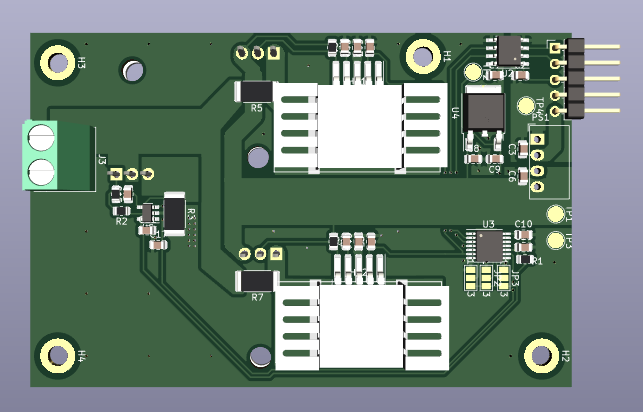
\includegraphics[width=0.45\textwidth]{pcb_cell_board_top.png}
    \caption{PCB layout of the top of the cell board.}
    \label{fig:pcb_top_cellboard}
\end{figure}
\FloatBarrier
\begin{figure}[h]
    \centering
    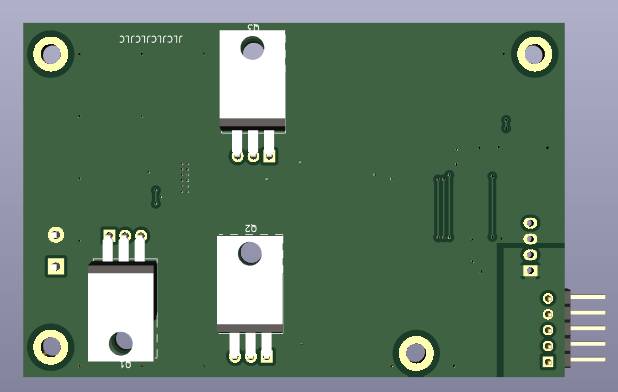
\includegraphics[width=0.45\textwidth]{pcb_cell_board_bottom.png}
    \caption{PCB layout of the bottom of the cell board.}
    \label{fig:pcb_bottom_cellboard}
\end{figure}
\FloatBarrier
\begin{figure}[h]
    \centering
    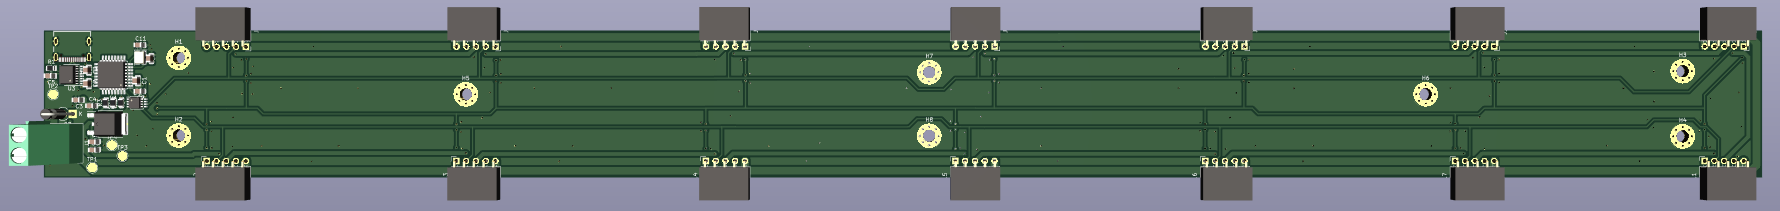
\includegraphics[width=0.45\textwidth]{pcb_model_board_top.png}
    \caption{PCB layout of the model board.}
    \label{fig:pcb_modelboard}
\end{figure}
\FloatBarrier